\documentclass[11pt,letterpaper]{article}
\usepackage[lmargin=1in,rmargin=1in,bmargin=1in,tmargin=1in]{geometry}
\usepackage{checkins}

\pgfplotsset{soldot/.style={color=black,only marks,mark=*},
		holdot/.style={color=black,fill=white,only marks,mark=*},
		compat=1.12
}

% -------------------
% Content
% -------------------
\begin{document}
\thispagestyle{title}

% 08/22
\checkin{08/22} If $\ds\lim_{x \to 5} f(x)= -3$, then $f(5)= -3$. \pspace

\sol The statement is \textit{false}. A function's limit (if it even exists) \textit{does not} have to be the same as the function's value at that limiting value---the function does not even have to be defined there! Consider the three examples below. \par
	\begin{center}
	% Left
	\fbox{%
	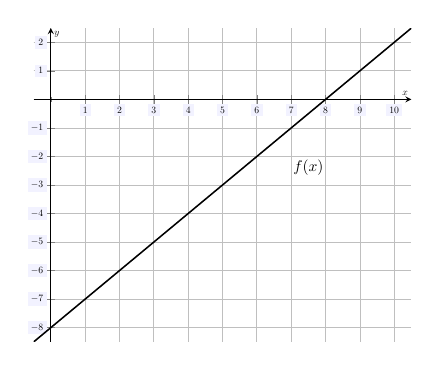
\begin{tikzpicture}[scale=0.7,every node/.style={scale=0.5}]
	\begin{axis}[
	grid=both,
	axis lines=middle,
	ticklabel style={fill=blue!5!white},
	xmin= -0.5, xmax=10.5,
	ymin= -8.5, ymax=2.5,
	xtick={-1,0,...,11},
	ytick={-8,-7,...,2},
	minor tick = {-9,-8,...,3},
	xlabel=\(x\),ylabel=\(y\),
	samples=20]
	\node at (7.5,-2.4) {\scalebox{1.6}{$f(x)$}};
	\addplot[thick, samples=5, domain= -0.5:10.5] {x - 8};
	\end{axis}
	\end{tikzpicture}
	} \hfill
	% Middle
	\fbox{%
	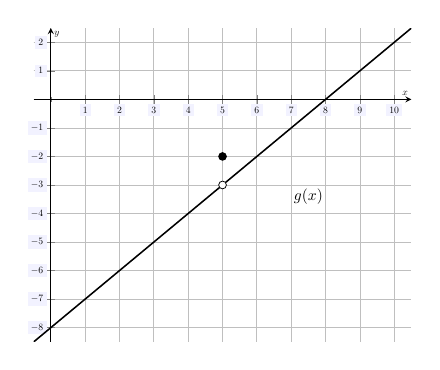
\begin{tikzpicture}[scale=0.7,every node/.style={scale=0.5}]
	\begin{axis}[
	grid=both,
	axis lines=middle,
	ticklabel style={fill=blue!5!white},
	xmin= -0.5, xmax=10.5,
	ymin= -8.5, ymax=2.5,
	xtick={-1,0,...,11},
	ytick={-8,-7,...,2},
	minor tick = {-9,-8,...,3},
	xlabel=\(x\),ylabel=\(y\),
	samples=20]
	\node at (7.5,-3.4) {\scalebox{1.6}{$g(x)$}};
	\addplot[thick, samples=5, domain= -0.5:10.5] {x - 8};
	\addplot[soldot] coordinates{(5,-2)};
	\addplot[holdot] coordinates{(5,-3)};
	\end{axis}
	\end{tikzpicture}
	} \hfill
	% Right
	\fbox{%
	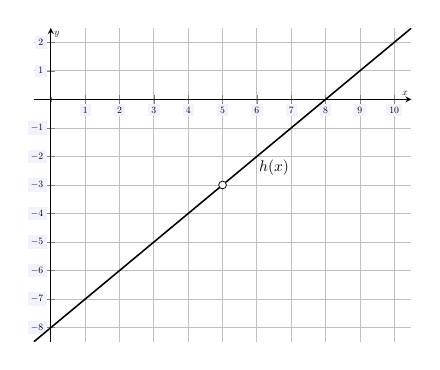
\begin{tikzpicture}[scale=0.7,every node/.style={scale=0.5}]
	\begin{axis}[
	grid=both,
	axis lines=middle,
	ticklabel style={fill=blue!5!white},
	xmin= -0.5, xmax=10.5,
	ymin= -8.5, ymax=2.5,
	xtick={-1,0,...,11},
	ytick={-8,-7,...,2},
	minor tick = {-9,-8,...,3},
	xlabel=\(x\),ylabel=\(y\),
	samples=20]
	\node at (6.5,-2.4) {\scalebox{1.6}{$h(x)$}};
	\addplot[thick, samples=5, domain= -0.5:10.5] {x - 8};
	\addplot[holdot] coordinates{(5,-3)};
	\end{axis}
	\end{tikzpicture}
	}
	\end{center} \par
For the graph of $f(x)$ on the left, $\ds\lim_{x \to 5} f(x)= -3$, so they are equal. However, observe that for $g(x)$ (the middle graph), we have $\ds\lim_{x \to 5} g(x)= -3$ but $g(5)= -2$, so that $\ds\lim_{x \to 5} g(x) \neq g(5)$. Similarly, in the graph of $h(x)$ on the right, $\ds\lim_{x \to 5} h(x)= -3$ but $h(-3)$ is not defined, so that $\ds\lim_{x \to 5} h(x) \neq h(-3)$. A function's value (if even defined) need not be related to its limit (if the limit even exists). \pvspace{1.3cm}



% 08/25
\checkin{08/25} The limit $\ds\lim_{x \to 0} \dfrac{\sin x}{x}= \text{DNE}$ because $\tfrac{\sin x}{x}$ becomes $\tfrac{0}{0}$ when one `plugs-in' $x= 0$ and $\frac{0}{0}$ is undefined. \pspace

\sol The statement is \textit{false}. In fact, $\ds\lim_{x \to 0} \dfrac{\sin x}{x}= 1$. Yes, $\tfrac{0}{0}$, $\pm\tfrac{\infty}{\infty}$, $0 \cdot \infty$, $\infty - \infty$, $0^0$, $1^\infty$, and $\infty^0$ are indeterminant/undefined expressions. However, that does not mean that the limit they arise from does not exist. The limit could exist or not---just like \textit{any} limit. `Running into' one of these expressions when evaluating a limit at its limiting value only means that one needs to try a different approach to determine if the limit exists or not. \pvspace{1.3cm}



% 08/27
\checkin{08/27} $\ds\lim_{x \to 0} \dfrac{\tan(5x)}{5x}= 1$ \pspace

\sol The statement is \textit{true}. Recall that $\ds\lim_{x \to 0} \dfrac{\sin(x)}{x}= 1$. We should think of this as $\ds\lim_{\Box \to 0} \dfrac{\sin \Box}{\Box}= 1$. But then\dots
	\[
	\lim_{x \to 0} \dfrac{\tan(5x)}{5x}= \lim_{x \to 0} \dfrac{\tfrac{\sin(5x)}{\cos(5x)}}{5x}= \lim_{x \to 0} \dfrac{\sin(5x)}{5x \cos x}= \lim_{x \to 0} \left( \dfrac{\sin(5x)}{5x} \cdot \dfrac{1}{\cos(5x)} \right)
	\]
Using the fact that $\ds\lim_{\Box \to 0} \dfrac{\sin \Box}{\Box}= 1$, we then have\dots
	\[
	\lim_{x \to 0} \dfrac{\tan(5x)}{5x}= \lim_{x \to 0} \left( \dfrac{\sin(5x)}{5x} \cdot \dfrac{1}{\cos(5x)} \right)= 1 \cdot \dfrac{1}{\cos(0)}= 1 \cdot \dfrac{1}{1}= 1
	\] \pvspace{1.3cm}

















\end{document}